\subsubsection{Examples}

\begin{frame}[fragile]
\frametitle{Classes in Simula}
%http://staff.um.edu.mt/jskl1/talk.html#Classes
\framesubtitle{}
A class in Simula consists of 4 parts, called:
%\begin{itemize}
%\item 
parameters, attributes, methods,
and  life (body). 
%\end{itemize}
\bigskip

\begin{cplus3}
! From the overview by J. Sklenar
! http://staff.um.edu.mt/jskl1/talk.html
Class Rectangle (Width, Height); Real Width, Height;
                           ! Class with two parameters;
 Begin
    Real Area, Perimeter;  ! Attributes;

    Procedure Update;      ! Methods (Can be Virtual);
    Begin
      Area := Width * Height;
      Perimeter := 2*(Width + Height)
    End of Update;

    Boolean Procedure IsSquare;
      IsSquare := Width=Height;

    Update;                ! Life of rectangle started at creation;
    OutText("Rectangle created: "); OutFix(Width,2,6);
    OutFix(Height,2,6); OutImage
 End of Rectangle;
\end{cplus3}
\end{frame}

\begin{frame}[fragile]
\frametitle{Classes in  Eiffel}
\framesubtitle{}
\begin{eiffel}
-- se.ethz.ch/teaching/ss2006/0050/slides/eiffel_the_essentials.pdf
indexing 
     description: "Representation of a book" 
class 
     BOOK 
create 
     make 
feature {NONE} -- Initialization 
     make (a_title: like title; some_authors: like authors) is 
          require 
                a_title_not_void: a_title /= Void 
                a_title_not_empty: not a_title.is_empty 
          do 
                title := a_title 
                authors := some_authors 
          ensure 
               title_set: title = a_title 
               authors_set: authors = some_authors 
          end 
feature -- Access 
     title: STRING 
invariant 
     title_not_void: title /= Void 
     title_not_empty: not title.is_empty 
end
\end{eiffel}
\end{frame}


\mycomment{
\begin{frame}[fragile]
\frametitle{More on constructors}
\framesubtitle{}
Name
\begin{itemize}
\item Predefined as in Java, \Cpp, C\#? Or any name, as in Eiffel?
\end{itemize}
Signature
\begin{itemize}
\item  Multiple constructors possible ($\leadsto$ overloading)? 
\end{itemize}
Definition
\begin{itemize}
\item 
Does the compiler create constructors (``default constructor'')? When? 
Can they be overridden?
\begin{eiffel}
-- Eiffel
default_create is
     do 
         create books.make
     end
// C++
class Point {
    int x, y;
public:
    Point(): x(0), y(0) {}
};    
\end{eiffel}
\end{itemize}
\end{frame}
}

\mycomment{
\begin{frame}[fragile]
\frametitle{Meta-classes in Smalltalk}
\framesubtitle{}
In Smalltalk, only objects can send messages.
What is the object that can send a 'creation' message? 
\begin{itemize}
\item Must belong to a class, but can't be of the same class. 
\end{itemize}
\bigskip

A \textit{meta-class} is a  class whose instances are classes.
\begin{itemize}
\item For every Smalltalk class, there exists a meta-class. The meta-classes
mirror the class hierarchy.
\item They specify how to create objects. 
\\ Examples:
\begin{java}
Time now.
   ``Answer a Time representing the time right now - is a 
     24 hour clock.''
Time new.
   ``Answer a Time representing midnight.''
Date today.
Data firstWeekdayOfMonth.
   ``Answer the weekday index of the first day in <month> 
     in the <year>.

\end{java}

\end{itemize}
\end{frame}
}


\section{A Quick Tour through Smalltalk}

\begin{frame}[fragile]
\frametitle{Smalltalk}
Material:
\begin{itemize}
  \item \url{http://www.squeak.org/Smalltalk}
  \item \url{http://squeakbyexample.org/SBE.pdf}
\end{itemize}

Principles
\begin{itemize}
\item Everything is an object.
\item All computation happens by sending \textit{messages} to objects:
\begin{cplus3}
      anObj aMethod: anArg
\end{cplus3}
\item Every object is an instance of a class.
\item All classes have a parent; \texttt{Object} is the root class.
\item All methods are public, all instance variables are private.
\end{itemize}


\end{frame}

\begin{frame}[fragile]
\frametitle{Smalltalk syntax}
% \url{http://www.mucow.com/squeak-qref.html} -- down
\begin{itemize}
\item Assignment
\begin{cplus3}
foo := 100 factorial.
\end{cplus3}

\item Messages
\begin{itemize}
\item Unary
\begin{cplus3}
4 factorial
'bla' asUppercase
Color yellow
\end{cplus3}

\item Infix syntax (``Binary'')
\begin{cplus3}
3 + 4
1 <= 10
3 + 4 * 2
\end{cplus3}

\item Named Arguments (``Keywords'')
\begin{cplus3}
nums := Array newFrom: (1 to: 5)
nums at: 1 put: \$a
nums at: 2 put: 3 + 4
\end{cplus3}
\end{itemize}
\end{itemize}
\end{frame}

\begin{frame}[fragile]
\frametitle{Blocks}
%http://daitanmarks.sourceforge.net/or/squeak/squeak_tutorial.html
Blocks %(a.k.a. block closure) 
correspond to anonymous functions. 

\begin{itemize}
\item They are objects (instances of \texttt{BlockContext}) and
typically receive the message \texttt{value:}.
\item They can have parameters (indicated by a leading colon):

\begin{cplus3}
[:x | 1 + x] value: 2
[:x :y | x + y] value: 1 value: 2
\end{cplus3}

\item They can  have local variables (indicated by bars):
\begin{cplus3}
[:x :y |  |z| z := x + y] value: 1 value:2 
\end{cplus3}

\item They can refer to variables of the surrounding scope
(they create \emph{closures}):
\begin{cplus3}
|newArray|
newArray :=  ... 
[:i | newArray at: i put: (aCollection at: i)]
\end{cplus3}
\end{itemize}

exercise: relate to λ-expression
\end{frame}

\begin{frame}[fragile]

\frametitle{Object models}
\framesubtitle{Layout in memory}
Value model:
\begin{itemize}
\item Variables (fields) stored as values, objects allocated directly
on run-time stack. Ex: \cpp, \textit{struct}s in C\#
%Ada, Modula-3
\end{itemize}

\begin{tabular}{ll}
\begin{minipage}{5cm}
\begin{cplus3}
public struct Poly { // C#
    public int deg;
    public myvector terms;
}
Poly p; 
p.deg = 
\end{cplus3}
\end{minipage}

& 

\begin{tabular}{l}
{\small 
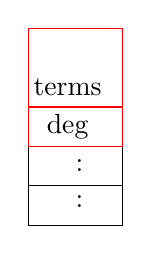
\begin{tikzpicture}
\draw (0,0)  rectangle (1.2,0.5);
\pgftext[at={\pgfpoint{0.65cm}{0.3cm}}]{:} ;
%\draw[->] (1.0, 0.1) .. controls (1.9, -0.2) and (2.5, 2.5) .. (3,1.5);

\draw (0,0.5)  rectangle (1.2,1.0);
\pgftext[at={\pgfpoint{0.65cm}{0.75cm}}]{:} ;


\draw[red] (0,1.0)  rectangle (1.2,1.5);
\pgftext[at={\pgfpoint{0.5cm}{1.25cm}}]{deg} ;


\draw[red] (0,1.5)  rectangle (1.2,2.5);
\pgftext[at={\pgfpoint{0.5cm}{1.75cm}}]{terms} ;

%\draw[red] (0,2.0)  rectangle (1.2,2.5);
%\pgftext[at={\pgfpoint{0.5cm}{1.75cm}}]{} ;


\end{tikzpicture}
}
\end{tabular}
\end{tabular}
%\bigskip

Reference model:
\begin{itemize}
%\item References are stored, object is allocated on the heap.
\item Run-time stacks holds a reference;  object (fields)
allocated on the heap.
Ex: Smalltalk (pure), Java/C\# : class inst's
\end{itemize}


%
\begin{tabular}{ll}
\begin{minipage}{4cm}

\end{minipage}

& 

\begin{tabular}{l}
{\small 
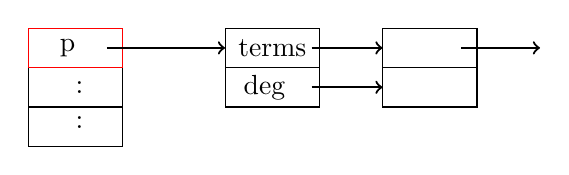
\begin{tikzpicture}
\draw (0,0)  rectangle (1.2,0.5);
\pgftext[at={\pgfpoint{0.65cm}{0.3cm}}]{:} ;
%\draw[->] (1.0, 0.1) .. controls (1.9, -0.2) and (2.5, 2.5) .. (3,1.5);

\draw (0,0.5)  rectangle (1.2,1.0);
\pgftext[at={\pgfpoint{0.65cm}{0.75cm}}]{:} ;


\draw[red] (0,1.0)  rectangle (1.2,1.5);
\pgftext[at={\pgfpoint{0.5cm}{1.25cm}}]{p} ;
\draw[->, thick] (1.0, 1.25) -- (2.5,1.25); 

%\draw (0,1.5)  rectangle (1.2,2.0);
%\pgftext[at={\pgfpoint{0.5cm}{1.75cm}}]{a: 4 } ;



% Object 
%\draw (3,0)  rectangle (4.2,0.5);
%\pgftext[at={\pgfpoint{3.5cm}{0.25cm}}]{prev} ;

\draw (2.5,0.5)  rectangle (3.7,1.0);
\pgftext[at={\pgfpoint{3.0cm}{0.75cm}}]{deg} ;
\draw[->, thick] (3.6, 0.75) -- (4.5,0.75); 
%
\draw (2.5,1.0)  rectangle (3.7,1.5);
\pgftext[at={\pgfpoint{3.1cm}{1.25cm}}]{terms} ;
\draw[->, thick] (3.6, 1.25) -- (4.5,1.25); 

% Object fields
\draw (4.5,0.5)  rectangle (5.7,1.5);
\draw[->, thick] (5.5, 1.25) -- (6.5,1.25); 
\draw (4.5,1.0)  rectangle (5.7,1.5);
%\pgftext[at={\pgfpoint{4.5cm}{1.25cm}}]{x: 3} ;


\end{tikzpicture}
}
\end{tabular}
\end{tabular}

Value model more efficient; reference model more flexible.

\end{frame}


\begin{frame}[fragile]
\frametitle{Curse of temporaries}
\framesubtitle{The costs of OOP}
How many objects are constructed?
\begin{cplus3}
     // C++
     typedef matrix<complex<float> > > matrix;
     matrix M = ...; // construct M
     matrix N = matrix(M);
     M = (M + N) * N;
\end{cplus3}
\bigskip

Intermediate objects (``temporaries'') are a practical problem:
\begin{itemize}
\item Run-time costs
\item Memory costs
\end{itemize}
\bigskip

Advanced techniques exist to avoid their creation.\\
If they must be created, at least  limit their lifetimes.
\end{frame}


\begin{frame}[fragile]
\frametitle{Automated deallocation and destruction}
\framesubtitle{}
Garbage collection
\begin{itemize}
\item Internal routine that automatically visits the heap, looks for
unused (``non-referenced) objects. 
\item Performs necessary finalization
and reclaims the memory.
\end{itemize}
Destructors 
\begin{itemize}
\item 
Based on blocks and scoping mechanisms: deallocation 
done automatically (when object leaves block = ``goes out of scope'').
\item Finalization: encapsulated in destructor. 
Destructor called automatically 
(when object goes out of scope).
\begin{cplus3}
// Example: C++ destructors  
class file {
public:
   file( const string&  name ) : file_handle(fopen(name, "w+")){}  
   ~file() { fclose(file_handle); }  // destructor
private:
   ...
};
\end{cplus3}
\end{itemize}
\end{frame}


Value model:

\begin{tabular}{ll}
\begin{minipage}{4cm}
\begin{cplus3}
class base {
   boolean b; 
   poly p;
}
class child extends base {
  integer c;
}
\end{cplus3}
\end{minipage}

& 

\begin{tabular}{l}
{\small 
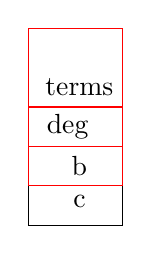
\begin{tikzpicture}
\draw (0,0)  rectangle (1.2,0.5);
\pgftext[at={\pgfpoint{0.65cm}{0.3cm}}]{c} ;
%\draw[->] (1.0, 0.1) .. controls (1.9, -0.2) and (2.5, 2.5) .. (3,1.5);

\draw[red] (0,0.5)  rectangle (1.2,1.0);
\pgftext[at={\pgfpoint{0.65cm}{0.75cm}}]{b} ;


\draw[red] (0,1.0)  rectangle (1.2,1.5);
\pgftext[at={\pgfpoint{0.5cm}{1.25cm}}]{deg} ;


\draw[red] (0,1.5)  rectangle (1.2,2.5);
\pgftext[at={\pgfpoint{0.65cm}{1.75cm}}]{terms} ;

%\draw[red] (0,2.0)  rectangle (1.2,2.5);
%\pgftext[at={\pgfpoint{0.5cm}{1.75cm}}]{} ;


\end{tikzpicture}
}
\end{tabular}
\end{tabular}

\bigskip

Reference model:

\begin{tabular}{ll}
\begin{minipage}{4cm}

\end{minipage}

& 

\begin{tabular}{l}
{\small 
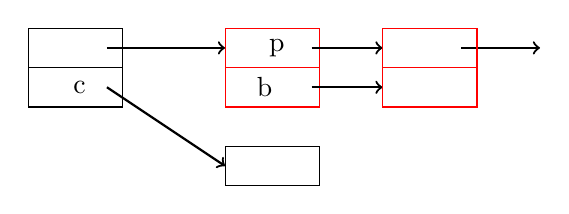
\begin{tikzpicture}
%\draw (0,0)  rectangle (1.2,0.5);
%\pgftext[at={\pgfpoint{0.65cm}{0.3cm}}]{:} ;
%\draw[->] (1.0, 0.1) .. controls (1.9, -0.2) and (2.5, 2.5) .. (3,1.5);

\draw (0,0.5)  rectangle (1.2,1.0);
\pgftext[at={\pgfpoint{0.65cm}{0.75cm}}]{c} ;
\draw[->, thick] (1.0, 1.25) -- (2.5,1.25); 

\draw(0,1.0)  rectangle (1.2,1.5);
\pgftext[at={\pgfpoint{0.5cm}{1.25cm}}]{} ;
\draw[->, thick] (1.0, 0.75) -- (2.5,-0.25); 




% Object 
\draw (2.5,-0.5)  rectangle (3.7,0.0);
\pgftext[at={\pgfpoint{3.0cm}{-0.25cm}}]{} ;

\draw[red] (2.5,0.5)  rectangle (3.7,1.0);
\pgftext[at={\pgfpoint{3.0cm}{0.75cm}}]{b} ;
\draw[->, thick] (3.6, 0.75) -- (4.5,0.75); 
%
\draw[red] (2.5,1.0)  rectangle (3.7,1.5);
\pgftext[at={\pgfpoint{3.1cm}{1.25cm}}]{ p} ;
\draw[->, thick] (3.6, 1.25) -- (4.5,1.25); 

% Object fields
\draw[red] (4.5,0.5)  rectangle (5.7,1.5);
\draw[->, thick] (5.5, 1.25) -- (6.5,1.25); 
\draw[red] (4.5,1.0)  rectangle (5.7,1.5);


\end{tikzpicture}
}
\end{tabular}
\end{tabular}

\end{frame}




American vs. Scandinavian semantics of overriding
\begin{itemize}
\item Refinement
\begin{itemize}
\item child's method called within the parent's method
\item Behavior of the parent method preserved
\end{itemize}
\item Replacement
\begin{itemize}
\item Parent method (may be) called within the child's method
\item Behavior of the parent might or might not be preserved 
\end{itemize}
\end{itemize}
\end{frame}


\section{Dynamic Binding}

\begin{frame}[fragile]

\frametitle{Dynamic binding and polymorphism}
\begin{center}
``poly'' (Greek): many
\end{center}
Polymorphic variable: 
\begin{itemize}
\item A variable with multiple types
\item In OOP: inheritance + subtyping (``is-a'') 
\end{itemize}
Combine:
\begin{itemize}
\item \textit{Dynamic} binding of methods
\item Polymorphic variables
\end{itemize}
$\Longrightarrow$ polymorphism in OOP 

\end{frame}

\begin{frame}[fragile]
\frametitle{The issue}
\framesubtitle{}
%
\begin{cplus3}
        // C# 
        class A {
            public void Foo() { Console.WriteLine("A::Foo()"); }
        }

        class B : A  {
            public new void Foo() { Console.WriteLine("B::Foo()"); }
        }

        class Test {
            static void Main(string[] args)
            {
                A a;
                B b;

                a = new A();
                b = new B();
                a.Foo();  // output --> "A::Foo()"
                b.Foo();  // output --> "B::Foo()"

                a = new B();
                a.Foo();  // output -->  ??
            }
        }
\end{cplus3}
% Output: "A::Foo()"
\begin{itemize}
\item Statically, $a$ of type $A$.
\item Dynamically, 
\end{itemize}
\end{frame}

\mycomment{
\begin{frame}[fragile]
\frametitle{Deferred classes in Eiffel}
\framesubtitle{}
\end{frame}
}


\mycomment{
\begin{frame}
\frametitle{Implementation, step 1: static type check}
\framesubtitle{``Call-by-value'' strategy for parameter passing} 
Assume a non-dynamic language.
How does the compiler process the invocation of, say, 
\texttt{anObj.foo(i,j-k)}? 
Its steps:
\begin{enumerate}
\item Evaluate \texttt{anObj} to get the class or object on which ``foo'' is
called.
\item Evaluate the (expressions for the) arguments $i$ and $j-k$ to obtain
the actual parameter values.
\item Create an \textit{activation record} with space for all formal
parameters and  push it on the run-time stack.
\item Initialize formal parameters with the values of the actual parameters.
\item Dispatch control to the method \texttt{anObj.foo}. 
\end{enumerate}
\end{frame}
}

\mycomment{
\begin{frame}
\frametitle{Implementation, step 2: dispatching}
Calling the right method: done through a run-time mechanism called 
\textit{dispatching}. Compiler does not generate code to call the method. Instead,
it generates code to find the right method:
\bigskip

Dispatching algorithm:
\begin{enumerate}
\item Deduce the static type, using variable and method declarations.
\item Keep dynamic type (from construction or assignment time).
\item Check whether static type is a supertype of dynamic type.
\item Check whether method is legal for static type.
\item Go to the object, retrieve the address of the code of its method;
generate code that branches to that address.
% Correct: go to vtbl
\end{enumerate}


\end{frame}
} % mycomment



\begin{frame}
\frametitle{Polymorphism in OOP}
Polymorphic variables in OOP are of reference type.
\begin{itemize}
\item In Java, Smalltalk, Eiffel: all variables are polymorphic.
\item In C\#, \Cpp, Ada: variables of value types are not polymorphic;
references are. 
\end{itemize}
\bigskip

Polymorphic = dynamically bindable methods (``virtual methods'') 
 
\begin{itemize}
\item In Java, Smalltalk, Eiffel: all method are polymorphic.
\item In Simula, C\#, \Cpp:  both virtual and non-virtual methods possible;
 keyword needed. 
\end{itemize}
% Return to C\# example
\end{frame}

\begin{frame}[fragile]
\frametitle{Type checking }
\framesubtitle{}
How to type-check if the method is not known before run time? 
\bigskip

Dynamic languages (Smalltalk, Ruby): 
\begin{itemize}
\item No type check (regardless of polymorphism), can get run-time error
\begin{cplus3}
       obj <- aMethod
\end{cplus3}
\end{itemize}

Non-dynamic languages (Java, C\#, \Cpp, Eiffel):

\begin{itemize}
\item Type check based on static type (why?).
\item If check succeeds on the static type, 
inheritance guarantees that method exists also for the dynamic
type 
\\
$\leadsto$ no run-time error

\begin{cplus3}
Base b = new Child();
b.foo()                // check or issue ``symbol not found''
\end{cplus3}
\end{itemize}

\end{frame}


\begin{frame}[fragile]
\frametitle{Dispatch vector (virtual function table)}

Dispatching requires an auxiliary data structure: the virtual function table
(a.k.a. dispatch vector).

\begin{itemize}
\item Every \textit{object} holds a reference to the function table.
\item The table is shared among all objects of a class.
\item It contains one entry per method (declared or inherited). The
entry stores the start address of the code of the method.
\end{itemize}

\bigskip
\begin{tabular}{ll}
\begin{minipage}{4.3cm}
\begin{cplus3}
class Foo {
  int i;
  boolean b;
  public void m1() {...}
  public Integer m2() {...}
  public Window m3() {..}
}
Foo f = new Foo();
\end{cplus3}
\end{minipage}

& 

\begin{tabular}{l}
{\small 
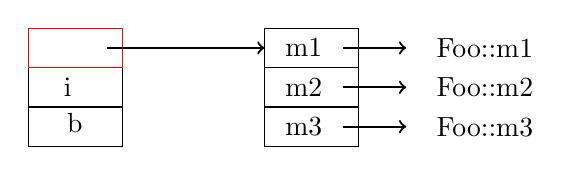
\begin{tikzpicture}
\draw (0,0)  rectangle (1.2,0.5);
\pgftext[at={\pgfpoint{0.65cm}{0.3cm}}]{b } ;
%\draw[->] (1.0, 0.1) .. controls (1.9, -0.2) and (2.5, 2.5) .. (3,1.5);

\draw (0,0.5)  rectangle (1.2,1.0);
\pgftext[at={\pgfpoint{0.5cm}{0.75cm}}]{i} ;


\draw[red] (0,1.0)  rectangle (1.2,1.5);
\pgftext[at={\pgfpoint{0.5cm}{1.25cm}}]{} ;
\draw[->, thick] (1.0, 1.25) -- (3.0,1.25); 





% right one 
\draw (3,0)  rectangle (4.2,0.5);
\pgftext[at={\pgfpoint{3.5cm}{0.25cm}}]{m3} ;
\draw[->, thick] (4.0, 0.25) -- (4.8,0.25); 
\pgftext[at={\pgfpoint{5.8cm}{0.25cm}}]{Foo::m3} ;

\draw (3,0.5)  rectangle (4.2,1.0);
\pgftext[at={\pgfpoint{3.5cm}{0.75cm}}]{m2} ;
\draw[->, thick] (4.0, 0.75) -- (4.8,0.75); 
\pgftext[at={\pgfpoint{5.8cm}{0.75cm}}]{Foo::m2} ;

\draw (3,1.0)  rectangle (4.2,1.5);
\pgftext[at={\pgfpoint{3.5cm}{1.25cm}}]{m1} ;
\draw[->, thick] (4.0, 1.25) -- (4.8,1.25); 
\pgftext[at={\pgfpoint{5.8cm}{1.25cm}}]{Foo::m1} ;

\end{tikzpicture}
}
\end{tabular}

\end{tabular}
\end{frame}




\begin{frame}[fragile]
\frametitle{Virtual function table and inheritance}
\framesubtitle{}
\begin{tabular}{ll}
\begin{minipage}{4.3cm}
\begin{cplus3}
class Foo {
  int i;
  boolean b;
  public void m1() {...}
  public Integer m2() {...}
  public Window m3() {..}
}
class Bar extends Foo {
  int y;

  // override
  public void m1() {..}

  // extend
  public int m4() {..}
}
Bar b = new Bar();
\end{cplus3}
\end{minipage}

& 

\begin{tabular}{l}
{\small 
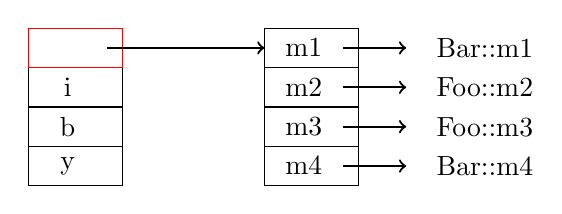
\begin{tikzpicture}

\draw (0,-0.5)  rectangle (1.2,0.0);
\pgftext[at={\pgfpoint{0.5cm}{-0.25cm}}]{y} ;

\draw (0,0)  rectangle (1.2,0.5);
\pgftext[at={\pgfpoint{0.5cm}{0.25cm}}]{b} ;


\draw (0,0.5)  rectangle (1.2,1.0);
\pgftext[at={\pgfpoint{0.5cm}{0.75cm}}]{i} ;


\draw[red] (0,1.0)  rectangle (1.2,1.5);
\pgftext[at={\pgfpoint{0.5cm}{1.25cm}}]{} ;
\draw[->, thick] (1.0, 1.25) -- (3.0,1.25); 





% right one 
\draw (3,-0.5)  rectangle (4.2,0.0);
\pgftext[at={\pgfpoint{3.5cm}{-0.25cm}}]{m4} ;
\draw[->, thick] (4.0, -0.25) -- (4.8,-0.25); 
\pgftext[at={\pgfpoint{5.8cm}{-0.25cm}}]{Bar::m4} ;


\draw (3,0)  rectangle (4.2,0.5);
\pgftext[at={\pgfpoint{3.5cm}{0.25cm}}]{m3} ;
\draw[->, thick] (4.0, 0.25) -- (4.8,0.25); 
\pgftext[at={\pgfpoint{5.8cm}{0.25cm}}]{Foo::m3} ;

\draw (3,0.5)  rectangle (4.2,1.0);
\pgftext[at={\pgfpoint{3.5cm}{0.75cm}}]{m2} ;
\draw[->, thick] (4.0, 0.75) -- (4.8,0.75); 
\pgftext[at={\pgfpoint{5.8cm}{0.75cm}}]{Foo::m2} ;

\draw (3,1.0)  rectangle (4.2,1.5);
\pgftext[at={\pgfpoint{3.5cm}{1.25cm}}]{m1} ;
\draw[->, thick] (4.0, 1.25) -- (4.8,1.25); 
\pgftext[at={\pgfpoint{5.8cm}{1.25cm}}]{Bar::m1} ;

\end{tikzpicture}
}
\end{tabular}

\end{tabular}
\end{frame}
